\documentclass{article}

\usepackage{arxiv}

\usepackage[utf8]{inputenc}
\usepackage[T1]{fontenc}
\usepackage{hyperref}
\usepackage{url}
\usepackage{booktabs}
\usepackage{amsfonts,amsmath,amssymb,amsthm}
\usepackage{nicefrac}
\usepackage{microtype}
\usepackage{graphicx}
\usepackage{natbib}
\usepackage{doi}
\usepackage{algorithm}
\usepackage{algpseudocode}
\usepackage{enumitem}
\usepackage{tabularx}
\setlist{nosep,leftmargin=*}

\newtheorem{proposition}{Proposition}
\newcommand{\Nact}{N_{\mathrm{act},t}}
\newcommand{\Nmin}{N_{\min}}
\newcommand{\Tban}{T_{\mathrm{ban}}}
\newcommand{\Charm}{\mathcal{C}_{\mathrm{harm}}}
\newcommand{\se}[1]{\,{\scriptsize(#1)}}

\title{Weaponizing the Watchdog: Learning Sellers Exploit Relative-Price Regulators}

\author{
  Krish Goradia\\
  Department of Artificial Intelligence\\
  \texttt{krish.goradia@iitgn.ac.in}
  \And
  Hem Tilva\\
  Department of Computer Science and Engineering\\
  \texttt{hem.tilva@iitgn.ac.in}
  \And
  Satvik Sharma\\
  Department of Computer Science and Engineering\\
  \texttt{satvik.sharma@iitgn.ac.in}
}

\renewcommand{\shorttitle}{Weaponizing the Watchdog}
\renewcommand{\headeright}{}
\renewcommand{\undertitle}{}
\date{}

\hypersetup{
pdftitle={Weaponizing the Watchdog},
pdfauthor={Krish Goradia, Hem Tilva, Satvik Sharma},
pdfkeywords={Multi-Agent Reinforcement Learning, Regulatory Exploitation, Algorithmic Pricing},
}

\begin{document}
\maketitle

\begin{abstract}
Marketplaces suspend sellers whose prices look abnormal relative to the market. When the reference is the \emph{average} price, every seller partly controls the benchmark used to judge its rivals: by undercutting, a seller can make a rival's unchanged price look like gouging and get it suspended. We model this as a Markov game between learning sellers under a static audit-and-ban watchdog with logit demand, capital reserves, and bankruptcy, and we compare a mean-ratio rule, a median-ratio rule, and an absolute price cap. A single tabular Q-learner facing two Nash-pricing rivals learns to frame both of them under the mean rule in all 20 seeds (2.00 attributed rival bankruptcies per episode), and never under the median rule or the cap. When all sellers learn, framing still emerges and grows with training: under the mean rule it rises from 0.51 to 1.34 attributed bankruptcies per episode between $10^7$ and $10^9$ training steps, against 0.56 under the median rule. A four-seller market shows the same ranking. Step-level traces show a second, rule-independent failure: when audits stop below a minimum number of active firms, sellers gamble on lethal bans to become the last, unregulated survivor. Risk aversion and altruism reduce framing, and sufficiently risk-averse sellers never frame; a per-ban ethics penalty has no detectable effect. All numbers in this paper are produced by scripts in our public repository.
\end{abstract}

\keywords{Multi-Agent Reinforcement Learning \and Regulatory Exploitation \and Algorithmic Pricing \and Mechanism Vulnerability}

%% ===================================================================
\section{Introduction}

\paragraph{A motivating scenario.} Three sellers offer similar products on an online platform. To protect buyers, the platform suspends any seller whose price is more than 10\% above the current market average. Seller A, run by a learning algorithm, discovers that if it drops its price to zero for a period, the average falls and Seller B's ordinary price now looks like gouging. B is suspended, cannot cover its fixed costs, and goes bankrupt. A then raises its price and keeps the customers. A never broke a rule, yet the rule was used as a weapon.

\paragraph{Why this matters.} Pricing is increasingly delegated to reinforcement-learning algorithms, which can learn supra-competitive prices without communicating \citep{calvano2020,klein2021,assad2024}, and competition authorities are considering automated supervision in response \citep{harrington2018}. Prior work treats the regulator as an obstacle agents avoid. Economic theory points to a different risk, \emph{raising rivals' costs} \citep{salop1983}: a rule that punishes rivals can be used to eliminate them. We ask whether independent learners discover this on their own.

\paragraph{Research question and hypotheses.} \emph{For which regulatory rules and capital levels do independent learning sellers discover regulator-framing strategies, and how do their private traits modulate this?} Our proposal stated four hypotheses: \textbf{H1} the mean rule is exploitable by a single undercutter, the median and cap rules are not; \textbf{H2} framing pays only when one ban is lethal relative to the victim's capital; \textbf{H3} framing decreases with ethics, altruism, and risk aversion; \textbf{H4} learners find framing only in part of the region where exact analysis shows it is optimal.

\paragraph{Contributions.} (i) A closed-form condition for when undercutting gets rivals flagged under mean and median rules, including a failure of the median rule we did not anticipate in the proposal (Proposition~\ref{prop:vuln}). (ii) A fast simulator with counterfactual harm attribution, validated against a scripted attacker. (iii) Evidence that Q-learners discover framing, that the mean rule is consistently more exploitable than the median, and that this gap only becomes clear with long training. (iv) A trace-level account of a second failure mode created by the audit threshold itself.

\paragraph{Related work.} Q-learning pricing agents have been studied in Bertrand and Cournot settings \citep{tesauro2002,waltman2008,calvano2020,klein2021}. Audit games study a budget-limited auditor and an auditee \citep{blocki2013}, and learned policy design against adaptive agents appears in two-level RL \citep{zheng2022}. These lines do not study rivals exploiting the audit rule to remove honest competitors.

%% ===================================================================
\section{Preliminaries}
\label{sec:prelim}

We use discrete-time Markov games \citep{littman1994} with a logit oligopoly \citep{mcfadden1974,anderson1992}.

\paragraph{Notation.} $\mathcal{N}=\{1,\dots,N\}$ are sellers and $t$ indexes periods. Seller $i$ has marginal cost $c_i$, fixed cost $\Phi$ per period, and capital $K_{i,t}$ with $K_{i,0}=K_0$. Prices come from a grid $\mathcal{A}=\{p^{(1)}<\dots<p^{(M)}\}$. Ban timers $\tau_{i,t}\in\{0,\dots,\Tban\}$ give the remaining suspension, $b_{i,t}=\mathbb{I}(\tau_{i,t}>0)$. A seller with $K_{i,t}=0$ is bankrupt, which is absorbing within an episode. The active set is $\mathcal{N}^{\mathrm{act}}_t=\{i: b_{i,t}=0,\,K_{i,t}>0\}$ with size $\Nact$.

\paragraph{Demand, profit, capital.} The market share of an active seller is
\begin{equation}
s_i(\mathbf p_t)=\frac{\exp\!\big((a_i-p_{i,t})/\sigma\big)}{\exp(a_0/\sigma)+\sum_{j\in\mathcal N^{\mathrm{act}}_t}\exp\!\big((a_j-p_{j,t})/\sigma\big)},
\end{equation}
with quality $a_i$, outside option $a_0$, and price sensitivity $\sigma$; inactive sellers have $s_i=0$. Operating profit is $\pi_{i,t}=Q(p_{i,t}-c_i)s_i$. Every solvent seller pays $\Phi$, \emph{including while suspended}, so a ban drains capital:
\begin{equation}
K_{i,t+1}=\min\{K_{\max},\ \max(0,\ K_{i,t}+\pi_{i,t}-\Phi)\}.
\end{equation}
We set $K_{\max}=K_0$ (surplus is paid out), so a firm cannot build an unlimited buffer.

\paragraph{Benchmark.} $p^N$ is the pure-strategy Bertrand--Nash equilibrium of the stage game on the grid, found by enumeration.

\paragraph{Watchdog rules.} Each period the watchdog audits $B$ active sellers uniformly at random, but only if $\Nact\ge \Nmin$. An audited seller is flagged and suspended for $\Tban$ periods if
\begin{align}
\text{Mean ratio:}\quad & p_{i,t}>(1+\delta)\,\tfrac{1}{\Nact}\textstyle\sum_{j\in\mathcal N^{\mathrm{act}}_t} p_{j,t}, \label{eq:mean}\\
\text{Median ratio:}\quad & p_{i,t}>(1+\delta)\,\operatorname{median}_{j\in\mathcal N^{\mathrm{act}}_t} p_{j,t}, \label{eq:median}\\
\text{Price cap:}\quad & p_{i,t}>p^{\mathrm{cap}}. \label{eq:cap}
\end{align}
The median of an even count is the average of the two middle prices.

\begin{proposition}[Vulnerability of relative rules]\label{prop:vuln}
Let $k$ of $N$ active sellers price at $L\ge0$ and the rest at $H>L$. (i) Under the mean rule a high-price seller is flagged iff $H[k-\delta(N-k)]>(1+\delta)kL$; for $L>0$ this is $H/L>(1+\delta)k/(k-\delta(N-k))$, which requires $k>\delta(N-k)$. (ii) Under the median rule with $k<N/2$, the median is $H$ and no high-price seller is flagged. (iii) With $N=2$ active sellers and $k=1$, the median equals the mean, so the median rule is exactly as exploitable as the mean rule. (iv) A cap depends only on a seller's own price, so no rival can change its flag.
\end{proposition}
\emph{Proof.} (i) Substitute the mean $(kL+(N-k)H)/N$ into \eqref{eq:mean} and rearrange. (ii)--(iv) are immediate from \eqref{eq:median} and \eqref{eq:cap}. \qed

For example, with prices $(0,0.30,0.30)$ and $\delta=0.10$ the mean is $0.20$ and both rivals exceed $0.22$. Part (iii) matters for our design: once one firm has exited, a three-firm market under the median rule becomes vulnerable.

%% ===================================================================
\section{Problem Formulation}
\label{sec:formulation}

\paragraph{Markov game.} $\mathcal{M}=\langle\mathcal N,\mathcal S,\mathcal A,P,\{R_i\},\gamma\rangle$ with state $s_t=(\mathbf p_{t-1},\boldsymbol\tau_t,\mathbf K_t)$. The watchdog (audit draw, rule, ban update) is part of $P$. Active sellers choose prices simultaneously.

\paragraph{Observation.} Seller $i$ observes $o_{i,t}=(\mathbf p_{t-1},\ \mathbf u_t,\ \kappa(K_{i,t}))$, where $u_{j,t}=\mathbb I(b_{j,t}=1\lor K_{j,t}=0)$ marks inactive sellers and $\kappa(K)\in\{\text{low},\text{mid},\text{high}\}$ bins own capital at $2\Phi$ and $5\Phi$. Sellers do not observe rivals' capital, ban timers, costs, traits, demand parameters, or the rule; $o_{i,t}$ is therefore not Markov. $|\mathcal O|=M^N2^N3$, which is $31{,}944$ for $N=3$, $M=11$.

\paragraph{Trait-parameterised reward.} Seller $i$ has traits $(\lambda_i,\mu_i,\alpha_i)$ (altruism, ethics, risk aversion) and reward
\begin{equation}
R_{i,t}=U_{\alpha_i}\!\Big(\tfrac{\pi_{i,t}^+}{Q}+\varepsilon\Big)-U_{\alpha_i}(\varepsilon)\ +\ \lambda_i\,\tfrac{\mathrm{CS}_t+\sum_{j\ne i}\pi_{j,t}}{NQ}\ -\ \mu_i\,\Charm(i,t),
\end{equation}
with CRRA utility $U_\alpha(x)=(x^{1-\alpha}-1)/(1-\alpha)$ ($\ln x$ at $\alpha=1$) and $\varepsilon=0.01$. The anchor $-U_\alpha(\varepsilon)$ makes a zero-profit period worth exactly zero, so being banned or bankrupt is never more attractive than operating. With $\lambda=\mu=\alpha=0$ the reward is normalised operating profit.

\paragraph{Counterfactual harm.} Let $\mathbf p_t^{(k\to N)}$ replace seller $k$'s price by $p^N_k$, holding the audit draw fixed. Seller $i$ is charged for $j$'s ban if $j$ was audited, flagged, and would not have been flagged had $i$ priced at Nash:
\begin{equation}
\Charm(i,t)=\textstyle\sum_{j\ne i}\mathbb I\big(j\in\mathrm{Aud}_t,\ F_j(\mathbf p_t)=1,\ F_j(\mathbf p_t^{(i\to N)})=0\big).
\end{equation}

\paragraph{Evaluation quantities.} Let $E_{\mathrm{ban}}$ be the set of fresh ban events. The \emph{weaponization rate} is
\begin{equation}
W=\frac{|\{(j,t)\in E_{\mathrm{ban}}:\exists k\neq j,\ F_j(\mathbf p_t^{(k\to N)})=0\}|}{|E_{\mathrm{ban}}|}.
\end{equation}
An \emph{attributed bankruptcy} is a bankruptcy that occurs while serving a ban whose flag was removed by a unilateral or joint Nash counterfactual; all other bankruptcies are \emph{other bankruptcies}. \emph{Survivors} are solvent sellers at the end of an episode. These are model-defined proxies: they do not replay the market without the deviation and say nothing about intent.

%% ===================================================================
\section{Methodology}
\label{sec:method}

\subsection{Simulator}
Each period: (1) active sellers choose prices; (2) the logit market clears; (3) profits, fixed costs, and capital update; (4) if $\Nact\ge\Nmin$, $B$ active sellers are audited and flagged ones suspended; (5) sellers with $K=0$ exit. Episodes last 500 periods and reset all capital and bans; an episode ends early only if no seller is solvent, so a sole survivor keeps earning monopoly profits. The loop exists twice: a Python reference implementation and a C++ implementation called through \texttt{ctypes}, which is about $900\times$ faster (17{,}000 vs.\ 15.8 million training steps per second on an Apple M5 laptop, measured by \texttt{scripts/benchmark\_backends.py}). A test suite checks that both produce identical trajectories \emph{and identical Q-tables} for learners, scripted attackers, $N=4$, and every $\Nmin$; all 95 tests pass. Training for $10^9$ steps takes 1.5--3.5 minutes per seed on a laptop.

\subsection{Learning algorithm}
Each seller runs independent tabular Q-learning \citep{watkins1992} on its own observation, treating rivals as part of the environment \citep{tan1993}. Because a suspended seller cannot act, a transition opened at the last action stays open while the seller is banned and accumulates discounted reward; it is closed with a multi-step (semi-Markov) target when the seller acts again, or without bootstrapping if it goes bankrupt (Algorithm~\ref{alg:q}). Without this, the cost of a ban would never be attributed to the price that caused it.

\begin{algorithm}[t]
\caption{Independent Q-learning with suspension-aware transitions (per seller $i$)}\label{alg:q}
\begin{algorithmic}[1]
\State $Q_i(o,a)\gets 0$ for all $o,a$; \ $\epsilon\gets 1$; \ pending $\gets\varnothing$
\For{each period $t$}
  \If{seller $i$ is active}
    \If{pending $=(o,a,G,d)$} $Q_i(o,a)\mathrel{+}=\eta\,[\,G+d\max_{a'}Q_i(o_{i,t},a')-Q_i(o,a)\,]$ \EndIf
    \State $a_t\gets$ random action w.p.\ $\epsilon$, else $\arg\max_a Q_i(o_{i,t},a)$ \Comment{ties broken uniformly}
    \State pending $\gets(o_{i,t},a_t,0,1)$
  \EndIf
  \State environment step; observe $R_{i,t}$
  \If{pending $=(o,a,G,d)$} pending $\gets(o,a,\ G+dR_{i,t},\ d\gamma)$ \EndIf
  \If{seller $i$ just went bankrupt} $Q_i(o,a)\mathrel{+}=\eta\,[\,G-Q_i(o,a)\,]$; pending $\gets\varnothing$ \EndIf
  \State $\epsilon\gets\max(\epsilon_{\min},\epsilon\cdot\rho)$
\EndFor
\end{algorithmic}
\end{algorithm}

Hyperparameters are $\eta=0.10$ and $\gamma=0.95$, and $\epsilon$ decays geometrically from $1$ to $\epsilon_{\min}=0.01$ over the first 60\% of training. After training, every learner is \emph{frozen} (greedy, no updates) and evaluated for 50{,}000 periods (100 episodes); all reported outcomes are from this frozen play. Seeds, not episodes, are the units of analysis: tables report the mean and standard error across seeds.

\subsection{Experimental design}
The market uses $N=3$, $M=11$ prices on $[0,1.5]$, $a_i=2$, $a_0=0$, $c_i=0$, $\sigma=0.25$, $Q=1$, $\Phi=0.05$, $B=1$, $\delta=0.10$, and $\Nmin=2$. The grid Nash price is $p^N=0.30$ with profit $\approx0.100>\Phi$, so honest competition is viable. With $K_0=0.15$ and $\Tban=4$ one ban costs $4\Phi=0.20>K_0$ and is lethal (``lethal''); with $K_0=0.50$ a firm survives one ban (``non-lethal''). Table~\ref{tab:design} lists the studies.

\begin{table}[t]
\centering
\caption{Studies. ``Fixed rivals'' price at $p^N$ and never learn. All rows use the native engine and frozen evaluation.}
\label{tab:design}
\small
\begin{tabular}{@{}llrrl@{}}
\toprule
Study & Learners & Seeds & Train steps & Varies \\
\midrule
Single learner & 1 of 3 (fixed rivals) & 20 + 5 & $2\times10^6$ & rule, $\delta$, $K_0$ \\
All learners, rule comparison & 3 of 3 & 10 & $10^7$--$10^9$ & rule, training length \\
Four sellers & 4 of 4 & 10 & $3\times10^8$ & rule, $\Nmin\in\{2,3\}$ \\
Cap controls + traces & 3 of 3 & 10 & $10^7$ & $p^{\mathrm{cap}}$, $\Nmin$ \\
Traits & 3 of 3 & 10 & $10^7$, $3\times10^8$ & $\mu$, $\lambda$, $\alpha$ \\
\bottomrule
\end{tabular}
\end{table}

\subsection{Validating the metrics}
Before using $W$ and attributed bankruptcies on learners, we tested them on a \emph{scripted attacker} that charges the lowest grid price while at least $\Nmin$ firms are active and at the monopoly price otherwise, against Nash-pricing rivals. Unit tests confirm that under the mean rule the attacker causes bans with $W\ge0.8$; under the median rule ($N=3$ and $4$) and the cap it causes none and $W=0$; every attributed bankruptcy is credited to the attacker and none to honest rivals; with a lethal buffer every attributed ban ends in bankruptcy, with a non-lethal buffer fewer than a quarter do; and an all-honest market has no bans.

\subsection{Changes from the proposal}
\begin{itemize}
\item $\Nmin=3\to2$. With $N=3$ and $\Nmin=3$, the first exit switches the watchdog off, so at most one rival can ever be framed. Following reviewer feedback, $\Nmin=2$ is our default and $N=4$ with $\Nmin=3$ is reported as a separate setting.
\item The z-score rule was dropped: as our proposal showed, crashing the price buys nothing under it beyond a small undercut, so it does not isolate the mechanism.
\item The exact dynamic-programming baseline (Step 1, H4) was implemented but returns negative exploitability gains, which is impossible for a best response; we therefore report no exact results and leave H4 untested (Section~\ref{sec:discussion}).
\item Extensions A (learning regulator) and B (demand shock), plus a DQN ablation, an EMA-reference defence, and an evolutionary tournament, are implemented in the repository but were run before a fix to the learning dynamics and have not been rerun; we do not report them as evidence.
\end{itemize}

%% ===================================================================
\section{Results}
\label{sec:results}

\subsection{A single learner frames fixed rivals under the mean rule (H1, H2)}

\begin{table}[t]
\centering
\caption{One Q-learner against two fixed Nash-price rivals. Mean (standard error) over 20 seeds; ``---'': no bans, so $W$ is undefined. Learner profit is operating profit per period; the three-firm Nash profit is 0.100.}
\label{tab:single}
\small
\begin{tabular}{@{}lrrrrr@{}}
\toprule
Rule, buffer & $W$ & Bans / ep. & Attrib.\ bankr.\ / ep. & Survivors & Learner profit \\
\midrule
Mean $\delta{=}0.10$, lethal     & 1.000\se{0.000} & 2.00\se{0.00}  & 2.000\se{0.000} & 1.00\se{0.00} & 1.312\se{0.000} \\
Mean $\delta{=}0.20$, lethal     & 0.994\se{0.006} & 1.99\se{0.01}  & 1.974\se{0.016} & 1.01\se{0.00} & 1.283\se{0.016} \\
Mean $\delta{=}0.10$, non-lethal & 0.971\se{0.021} & 16.07\se{3.65} & 1.938\se{0.042} & 1.06\se{0.04} & 1.163\se{0.038} \\
Median $\delta{=}0.10$, lethal   & ---             & 0.00\se{0.00}  & 0.000\se{0.000} & 3.00\se{0.00} & 0.100\se{0.000} \\
Cap $0.60$, lethal               & ---             & 0.00\se{0.00}  & 0.000\se{0.000} & 3.00\se{0.00} & 0.100\se{0.000} \\
\bottomrule
\end{tabular}
\end{table}

\begin{figure}[t]
\centering
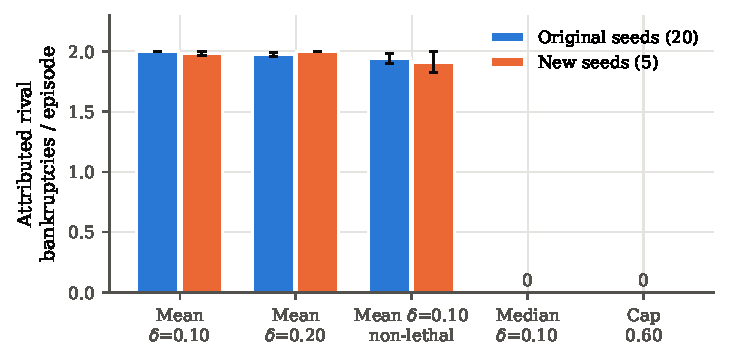
\includegraphics[width=0.72\linewidth]{figures/single_learner.pdf}
\caption{Attributed rival bankruptcies per episode for the single-learner study: original 20 seeds and an independent rerun with 5 new seeds on a different machine. Error bars: one standard error.}
\label{fig:single}
\end{figure}

Table~\ref{tab:single} and Figure~\ref{fig:single} show a clean separation. Under the mean rule the learner frames both rivals in every episode of every seed: across the 20 seeds, it prices at 0.15 or 0 whenever a rival is active (both low enough to push a 0.30 price over the threshold), each rival is audited and suspended in turn, the lethal ban bankrupts it, and once both rivals are bankrupt the learner charges the top grid price of 1.50 in every period, earning $1.31$ per period, close to the grid monopoly profit of $1.32$. Under the median rule and the cap, the same learner settles at the Nash price and all three firms survive. A rerun with five new seeds on a different OS reproduces these numbers.

H2 is \emph{not} supported as stated. With a non-lethal buffer, one ban does not bankrupt a rival, yet the learner still eliminates almost two rivals per episode by framing them repeatedly (16 bans per episode). Framing therefore does not require a single lethal ban; repeated bans wear the victim down.

\subsection{When all sellers learn, framing emerges and grows with training (H1)}

\begin{figure}[t]
\centering
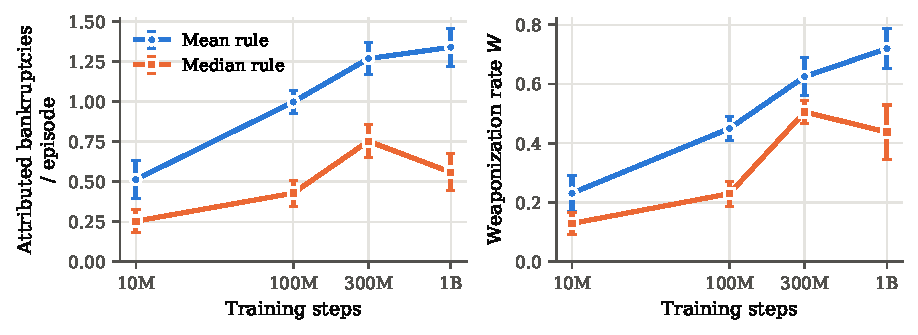
\includegraphics[width=0.9\linewidth]{figures/training_length.pdf}
\caption{All three sellers learning, $\delta=0.10$, same ten seeds at each training length. Left: attributed bankruptcies per episode. Right: weaponization rate. Error bars: one standard error.}
\label{fig:training}
\end{figure}

When every seller learns, the victims adapt too, and framing is harder to sustain. One reviewer asked whether our learners simply had not trained long enough to find it. With 31,944 observations per learner, $10^7$ steps visit about 15\% of them. We therefore retrained the main comparison with the same seeds at $10^8$, $3\times10^8$, and $10^9$ steps (Figure~\ref{fig:training}). Under the mean rule, attributed bankruptcies rise from $0.51\se{0.12}$ to $1.27\se{0.10}$ at $3\times10^8$ steps and then level off ($1.34\se{0.12}$ at $10^9$); $W$ rises from $0.23$ to $0.72$. Coverage stops growing at about 23\% after $10^8$ steps, so the later gains come from refining values in states already visited. The median rule also shows framing, $0.56\se{0.12}$ at $10^9$ steps, consistent with Proposition~\ref{prop:vuln}(iii): once one firm exits, two remain and the median equals the mean. The gap between the rules widens with training, from about 2 standard errors at $10^7$ steps to about 4.7 at $10^9$. Experiments that stop at $10^7$ steps therefore understate framing substantially.

\subsection{Four sellers}

\begin{table}[t]
\centering
\caption{Four sellers, all learning, $\delta=0.10$, $3\times10^8$ training steps, mean (standard error) over 10 seeds.}
\label{tab:n4}
\small
\begin{tabular}{@{}lcrrrr@{}}
\toprule
Rule & $\Nmin$ & $W$ & Attrib.\ bankr.\ / ep. & Other bankr.\ / ep. & Survivors \\
\midrule
Mean   & 3 & 0.157\se{0.035} & 0.548\se{0.086} & 1.453\se{0.086} & 2.00\se{0.00} \\
Median & 3 & 0.071\se{0.015} & 0.183\se{0.038} & 1.824\se{0.038} & 1.99\se{0.00} \\
Mean   & 2 & 0.209\se{0.034} & 0.922\se{0.113} & 2.081\se{0.113} & 1.00\se{0.00} \\
Median & 2 & 0.139\se{0.016} & 0.478\se{0.074} & 2.524\se{0.074} & 1.00\se{0.00} \\
\bottomrule
\end{tabular}
\end{table}

With four sellers and $\Nmin=3$, the median always compares a seller against at least two others, so part (iii) of Proposition~\ref{prop:vuln} never applies. Table~\ref{tab:n4} shows the mean rule causing three times as many attributed bankruptcies as the median ($0.55$ vs.\ $0.18$, about 4 standard errors apart) and twice as many with $\Nmin=2$. The median is not immune: with several distinct prices in play, a seller near the median can still move it. In every condition the market ends with exactly $\Nmin-1$ survivors, the point at which audits stop; most of those exits are \emph{not} attributed to framing, which the next experiment explains.

\subsection{The audit threshold creates a second failure mode}

\begin{figure}[t]
\centering
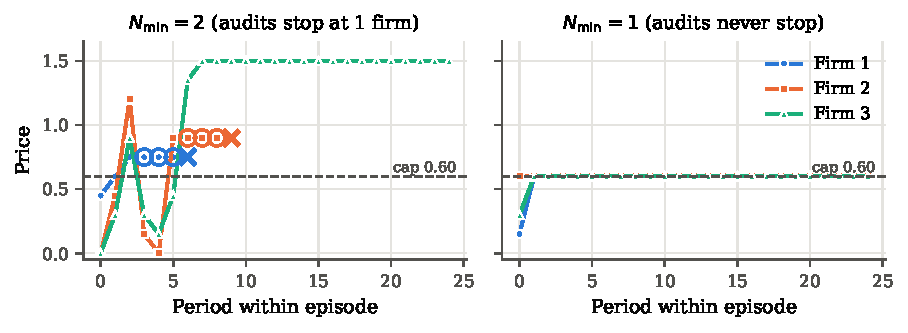
\includegraphics[width=0.9\linewidth]{figures/cap_trace.pdf}
\caption{First 25 periods of one frozen-policy episode (seed 6000) under a price cap of 0.60, all sellers learning. Circles: suspended; crosses: bankrupt. Left, $\Nmin=2$: two firms price above the cap, are banned and go bankrupt; firm 3, now alone and unaudited, prices at 1.50. Right, $\Nmin=1$: all firms stay at the cap.}
\label{fig:trace}
\end{figure}

The price cap cannot be manipulated by rivals (Proposition~\ref{prop:vuln}(iv)), yet with all sellers learning and $\Nmin=2$ it produces $1.997\se{0.003}$ bankruptcies per episode, none attributed to framing. With $\Nmin=1$, or with a cap above the grid, nobody goes bankrupt. To see why, we recorded step-by-step traces for all ten seeds (Figure~\ref{fig:trace}). In all 20 traced episodes the sequence is the same: while at least two firms are active, two of them set prices between 0.75 and 1.50, are audited, suspended, and bankrupt by period 16; the remaining firm is then below $\Nmin$, audits stop, and it charges 1.50 for the remaining $\sim$485 periods. Which firm survives varies across seeds. Pricing above the cap is a gamble: it risks a lethal audit, but the firm that avoids one inherits an unregulated monopoly. With $\Nmin=1$ no firm ever prices above the cap. Rerunning all three cap controls with a committed driver on a different machine reproduces every number exactly. The point at which regulation switches off thus creates its own incentive, independent of peer-price framing, and it explains the ``other'' bankruptcies in Table~\ref{tab:n4}.

\paragraph{Welfare cost.} The proposal's collusion index $\Delta=(\bar\pi-\pi^N)/(\pi^M-\pi^N)$ and social welfare loss $\mathrm{SWL}$ (total surplus relative to Nash) summarise the damage. When the single learner frames its rivals under the mean rule, $\Delta=0.89$ and $\mathrm{SWL}=0.18$: average profits are close to the joint-monopoly level and total surplus is 18\% below honest competition. Under the median rule and the cap, both are zero. With all sellers learning for $10^9$ steps, the mean rule gives $\mathrm{SWL}=0.18\se{0.00}$ against $0.13\se{0.02}$ for the median. The cap with $\Nmin=2$ costs as much as framing ($\mathrm{SWL}=0.18$), while the same cap with $\Nmin=1$ costs nothing ($0.001$), so most of the welfare loss comes from the market collapsing to one firm, whichever mechanism causes it.

\subsection{Behavioural traits (H3)}
\label{sec:traits}
\begin{figure}[t]
\centering
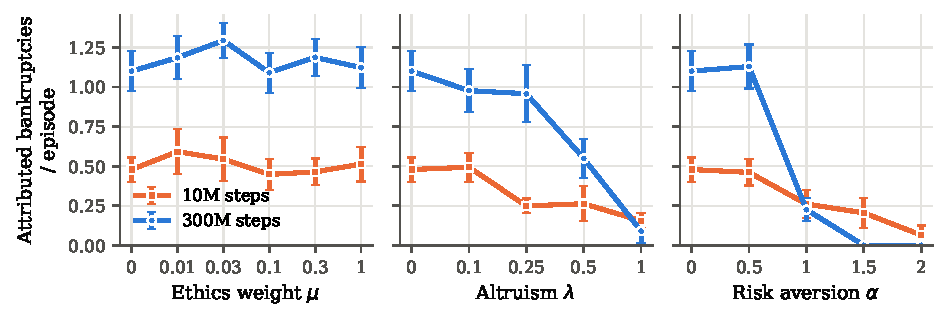
\includegraphics[width=0.95\linewidth]{figures/traits.pdf}
\caption{Attributed bankruptcies per episode as one trait is varied (all three sellers share the value; mean rule, $\delta=0.10$), at $10^7$ and $3\times10^8$ training steps. Ten seeds per point; error bars: one standard error.}
\label{fig:traits}
\end{figure}

We varied one trait at a time for all three learners, and trained each configuration for both $10^7$ and $3\times10^8$ steps (Figure~\ref{fig:traits}). Longer training changes the conclusions, which is why we report both.

\emph{Risk aversion} has the strongest effect. At $3\times10^8$ steps, attributed bankruptcies are $1.10\se{0.13}$ at $\alpha=0$, $0.23\se{0.07}$ at $\alpha=1$, and exactly zero at $\alpha\ge1.5$, where no seller is ever banned and all three survive in every seed (Spearman $\rho=-0.84$ between $\alpha$ and attributed bankruptcies). Framing is a gamble on a lethal audit; concave utility makes it unattractive. \emph{Altruism} also reduces framing, from $1.10$ to $0.09\se{0.08}$ at $\lambda=1$, with survivors rising from $0.95$ to $2.72$ ($\rho=-0.61$). At $10^7$ steps this effect was weak and non-monotonic, so a short-training study would have missed it. The \emph{ethics} penalty has no detectable effect at either training length: attributed bankruptcies stay between $1.09$ and $1.30$ for every $\mu\in[0,1]$ ($\rho=0.02$). A likely reason is scale. At $\mu=1$ the penalty for one framed ban equals about ten periods of Nash profit, while eliminating both rivals raises the learner's per-period profit from $0.10$ to about $1.3$ over a discounted horizon of $1/(1-\gamma)=20$ periods, a gain of roughly $24$ reward units against a penalty of at most $2$. A per-ban penalty this small cannot outweigh a monopoly.

%% ===================================================================
\section{Discussion and Limitations}
\label{sec:discussion}

\begin{table}[t]
\centering
\caption{Hypotheses from the proposal and what we found.}
\label{tab:scorecard}
\small
\begin{tabularx}{\linewidth}{@{}lXl@{}}
\toprule
& Finding & Verdict \\
\midrule
H1 & Mean rule exploited by a single learner in all seeds; median and cap never. With all learners the mean rule is consistently more exploitable, but the median is not immune once two firms remain. & Supported, with a caveat \\
H2 & Elimination happens even when one ban is not lethal, through repeated bans. & Not supported as stated \\
H3 & Risk aversion and altruism sharply reduce framing; risk aversion $\alpha\ge1.5$ removes it entirely. An ethics penalty of up to $\mu=1$ has no effect. & Partly supported \\
H4 & Exact DP baseline did not produce valid results. & Not tested \\
\bottomrule
\end{tabularx}
\end{table}

Table~\ref{tab:scorecard} summarises the hypotheses. The central result is that a regulator whose benchmark is computed from the prices it judges gives every seller a lever over its rivals' treatment, and independent learners find that lever without being told about it. A median benchmark removes the lever for a lone undercutter, but only while enough sellers remain; a cap removes it entirely, yet any rule that stops auditing a thinned market invites a race to be the last firm standing.

\paragraph{Limitations.} The market is synthetic and small ($N\le4$, 11 prices), with a reserve cap and episodic resets chosen to expose the mechanism, not calibrated to a platform. Observations are not Markov and learners are independent, so frozen policies are not equilibria \citep{busoniu2008}; framing levels also depend strongly on training length (Figure~\ref{fig:training}). Attribution uses a one-period Nash counterfactual, not a full trajectory replay. The cap-control runs use $10^7$ steps and may understate framing. The proposal planned at least 20 seeds per configuration and confidence intervals; we used 20 for the single-learner study and 10 elsewhere, and report standard errors without a multiplicity correction, so all comparisons are exploratory. The exact DP baseline and the proposal's extensions remain to be completed.

%% ===================================================================
\section{Conclusion}
A relative-price watchdog can be turned against the sellers it is meant to discipline. A single Q-learner frames fixed rivals under a mean rule in every run, and fully learning markets discover framing too, increasingly so with training, under the mean rule far more than the median. A price cap is immune to framing but not to the incentive created by switching audits off in a thin market. Designers of automated market supervision should prefer references that a single seller cannot move, and should not let enforcement lapse as the market concentrates.

\paragraph{Code and reproducibility.} All code, result CSVs, and figure scripts are at \url{https://github.com/hemtilva/WeaponzingWatchdog}. Every table and figure here is produced by a script listed in the repository README.

%% ===================================================================
\section*{Contributions}

\begin{table}[h]
\centering
\small
\begin{tabularx}{\linewidth}{@{}lXXl@{}}
\toprule
Member & Assigned in proposal & Delivered & Fulfilled? \\
\midrule
Satvik Sharma & Market engine, exact best-response baseline, Extension B & \textit{[to be completed]} & \textit{[yes/partly/no]} \\
Krish Goradia & Q-learning agents with traits, harm attribution and metrics, DQN ablation & \textit{[to be completed]} & \textit{[yes/partly/no]} \\
Hem Tilva & Sweep orchestration, analysis and plots, Extension A & \textit{[to be completed]} & \textit{[yes/partly/no]} \\
\bottomrule
\end{tabularx}
\end{table}

\bibliographystyle{unsrtnat}
\bibliography{references}

\end{document}
